\documentclass[oneside,10pt]{article}
\usepackage{pdfpages}
\usepackage[spanish]{babel}
\usepackage[a4paper]{geometry}
\usepackage{lipsum}
\usepackage{blindtext}
\usepackage[hidelinks]{hyperref}
\usepackage{tcolorbox}
\usepackage{multicol}

\usepackage[T1]{fontenc}
\usepackage{helvet}

\usepackage{fancyhdr}

%----------------------------------------------------------
% Esto modifica el índice para que figuren los autores

\newcommand{\desctotoc}[1]{%
	\addtocontents{toc}{\hspace*{1em}\medskip\detokenize{\textit{#1}}\leavevmode\par\medskip\vspace{-1.5em}}
}

\makeatletter
\let\latexl@section\l@section
\def\l@section#1#2{\begingroup\let\numberline\@gobble\latexl@section{#1}{#2}\endgroup}
\makeatother
%----------------------------------------------------------

%----------------------------------------------------------
% Geometría

\geometry{verbose,tmargin=2cm,bmargin=2cm,lmargin=2.5cm,rmargin=2.5cm}
%----------------------------------------------------------

\begin{document}
	
	%------------------------------------------------------------------------------------------------------------
	% Toda la primer parte
	
\includepdf{Portada.pdf}
	
	\clearpage
	
	\thispagestyle{empty}
	\begin{center}
	\LARGE \bfseries \sffamily
	Memorias de las VI Jornadas de Enseñanza de la Matemática (JEM)
\end{center}

\vspace*{2.5mm}

\begin{center}
	\begin{tcolorbox}[colback=white, arc=0mm, width=10cm, boxrule=0.5pt]
		\footnotesize
		Universidad Nacional de Salta
		
		\hspace*{1em} Memorias de las VI Jornadas de Enseñanza de la Matemática (JEM) / Compilado por Sángari, Antonio Noé - Salta: Universidad Nacional de Salta, 2023.
		
		\vspace*{1em}
		
		\hspace*{1em} Archivo digital: descarga y online
		
		\hspace*{1em} ISBN 978-987-633-615-4		
	\end{tcolorbox}
\end{center}

\vspace*{2.5mm}

\begin{center}
	\sffamily \Large \bfseries Compiladores
	
	\large \normalfont
	Guzmán González, Ramiro 
	
	Sángari, Antonio Noé 
\end{center}

\begin{center}
	\sffamily \Large \bfseries Revisores de talleres y comunicaciones breves
	
	\vspace*{-1em}
	
	\begin{multicols}{2}
		\large \normalfont
		Alberto, Diego Luis
		
		Aliendro, Estela Sonia
		
		Arias, Jesús Eduardo
		
		Ávila, Mario Ubaldo
		
		Bifano, Fernando Jorge  
		
		Duarte, Betina
		
		Etchegaray, Silvia Catalina
		
		Ferrero, María Martha 
		
		Formeliano, Blanca Azucena 
		
		Funes, Héctor Nicolás
		
		García, José Ignacio
		
		Martínez, Rosa
		
		Marrón, Beatriz Susana
		
		Méndez, Nilda Graciela
		
		Mercau, Beatriz Susana
		
		Oliva, Elisa
		
		Quintana, Pablo
		
		Rodríguez, Mabel Alicia
		
		Roig, María Eugenia 
		
		Rosales, Juan Carlos
		
		Puca, Silvana Mercedes del Milagro 
		
		Saidón, Liliana
		
		Sángari, Antonio Noé 
		
		Micelli, Mónica Lorena
		
		Torres, Germán Ariel
		
		Villagra, Celia Elizabeth
		
		Villarreal Cantizana, Claudia
		
		Viola, Fernanda Beatriz 
		
		Yazlle, Jorge Fernando
	\end{multicols} 
\end{center}

\begin{center}
	\sffamily \Large \bfseries Maquetación
	
	\large \normalfont
	Martinez, Gonzalo Matias
\end{center}

\begin{center}
	\sffamily \Large \bfseries Diseño e identidad
	
	\large \normalfont
	Díaz, Aldana Lucía
\end{center}

\vspace*{2.5mm}

\begin{center}
	\scshape \Large Universidad Nacional de Salta
	
	\normalfont \normalsize
	Av. Bolivia 5150 -- Salta Capital
\end{center}

\vfill

\begin{center}
	\footnotesize
	Queda prohibida la reproducción total o parcial del texto de la presente obra en cualquiera de sus formas, electrónica o mecánica, sin el consentimiento previo y escrito del autor.
\end{center}
	
	\clearpage
	
	\thispagestyle{empty}
	\begin{center}
	\LARGE \bfseries \sffamily Autoridades
\end{center}

\begin{center}
	\sffamily \Large \bfseries Universidad Nacional de Salta

	\bigskip
	
	\sffamily \large \bfseries Rector
	
	\normalfont \large
	Ing. Daniel HOYOS
	
	\bigskip
	
	\sffamily \large \bfseries Vicerrector
	
	\normalfont \large
	Cr. Nicolás INNAMORATO
	
	\bigskip
	
	\sffamily \large \bfseries Secretario de Extensión 
	
	\normalfont \large
	Lic. Rubén Emilio CORREA
\end{center}

\vspace*{5mm}

\begin{center}
	\sffamily \Large \bfseries Facultad de Ciencias Exactas
	
	\bigskip
	
	\sffamily \large \bfseries Decano
	
	\normalfont \large
	Mg. Gustavo Daniel GIL
	
	\bigskip
	
	\sffamily \large \bfseries Vicedecana
	
	\normalfont \large
	Dra. María Rita MARTEARENA
\end{center}

\vspace*{5mm}

\begin{center}
	\sffamily \Large \bfseries Departamento de Matemática
	
	\bigskip
	
	\sffamily \large \bfseries Directora
	
	\normalfont \large
	Lic. María Cristina AHUMADA
	
	\bigskip
	
	\sffamily \large \bfseries Secretario
	
	\normalfont \large
	Prof. Juan Pablo DIOLI
	
	\bigskip
	
	\sffamily \large \bfseries Prosecretario
	
	\normalfont \large
	Mg. Héctor Nicolás FUNES
\end{center}
	
	\clearpage
	
	\thispagestyle{empty}
	\begin{center}
	\LARGE \bfseries \sffamily Equipo Editorial JEM
\end{center}

\begin{center}
	\sffamily \Large \bfseries Coordinación General
	
	\bigskip
	
	\normalfont \large
	Prof. Silvia Mabel Baspiñeiro
	
	Prof. Blanca Azucena Formeliano
	
	Prof. lvone Anahí Patagua
	
	Prof. Antonio Noé Sángari
\end{center}

\vspace*{2.5mm}

\begin{center}
	\sffamily \Large \bfseries Plataforma
	
	\bigskip
	
	\sffamily \large \bfseries Open Journal System (OJS)
	
	\normalfont \large
	Lic. Ramiro Guzmán González
	
	\bigskip
	
	\sffamily \large \bfseries Diseño de Identidad
	
	\normalfont \large
	Lic. Aldana Lucía Díaz
	
	\bigskip
	
	\sffamily \large \bfseries Maquetación 
	
	\normalfont \large
	Gonzalo Matias Martinez
\end{center}

\vspace*{5mm}

\begin{center}
	\sffamily \Large \bfseries Declaraciones de Interés Educativo y Avales Institucionales
	
	\bigskip
	
	\normalfont \normalsize \scshape
	Rectorado
	
	Universidad Nacional de Salta
	
	RES. R. N° 937/2022
	
	\bigskip
	
	Facultad de Ciencias Exactas 
	
	Universidad Nacional de Salta
	
	RESD-EXA N° 379/2022
	
	\bigskip
	
	Ministerio de Educación, Cultura, Ciencia 
	
	y Tecnología de la Provincia de Salta
	
	RES. N° 128/2022
	
\end{center}
	
	\clearpage
	
	\section*{\centering \sffamily Prólogo}

Las VII Jornadas de Enseñanza de la Matemática híbridas, realizadas en su parte presencial en las instalaciones de la Universidad Nacional de Salta del 24 de julio al 2 de agosto de 2023, representaron un hito en el continuo esfuerzo por mejorar la calidad de la educación matemática en nuestra región. Durante esos días, docentes, investigadores y estudiantes se congregaron con el objetivo de reflexionar sobre sus prácticas docentes, compartiendo experiencias y conocimientos que, sin duda, contribuirán al enriquecimiento de la comunidad educativa.

Las Jornadas ofrecieron un variado programa de actividades que incluyó conferencias magistrales, talleres prácticos y comunicaciones breves. Entre las actividades destacadas, se encuentran las conferencias de Valeria Borsani, que abordó \emph{El pasaje de la aritmética al álgebra en los primeros años de la escuela media}, la de Andrés Rieznik, que abordó \emph{Discalculia, un capítulo olvidado de la neuropsicología}, y el de Daniela Reyes, \emph{Empoderamiento docente, ¿por qué pensar en ello?} y cinco talleres sobre enseñanza de la matemática. La participación activa de los asistentes reflejó el interés y el compromiso con la mejora continua de la enseñanza de la matemática.

Queremos expresar nuestro más sincero agradecimiento a todos los participantes, ponentes y talleristas que, con su dedicación y entusiasmo, hicieron posible el éxito de este evento. Asimismo, extendemos nuestro reconocimiento a la Universidad Nacional de Salta y a todas las instituciones que nos brindaron su apoyo.

Las presentes Memorias recogen las ideas, debates y conclusiones surgidas durante las Jornadas, sirviendo como un valioso recurso para todos aquellos interesados en la enseñanza de la matemática. Esperamos que este compendio inspire a los lectores a continuar explorando y aplicando nuevas estrategias pedagógicas en sus aulas.

Con la mirada puesta en el futuro, confiamos en que las próximas ediciones de las Jornadas de Enseñanza de la Matemática seguirán siendo un espacio de encuentro, reflexión e innovación para nuestra comunidad.

\vspace{5cm}

\begin{center}
	\large Prof. Antonio Noé Sángari
	
	\normalfont Coordinador de las VII Jornadas de Enseñanza de la Matemática
\end{center}
	
	\clearpage
	
	\tableofcontents
	
	\clearpage
	%------------------------------------------------------------------------------------------------------------
	
	%------------------------------------------------------------------------------------------------------------
	% Talleres
	\clearpage
	\vspace*{\fill}
	\begin{center}
		\sffamily \scshape \bfseries \LARGE I
		
		\Huge Talleres
	\end{center}
	\vspace*{\fill}
	\addcontentsline{toc}{part}{I \hspace*{1em} Talleres}
	\clearpage
	
	\fancyhead[C]{\small \scshape Memorias de las VI JEM}
	\fancyhead[R]{}
	\fancyfoot[C]{\thepage}
	
	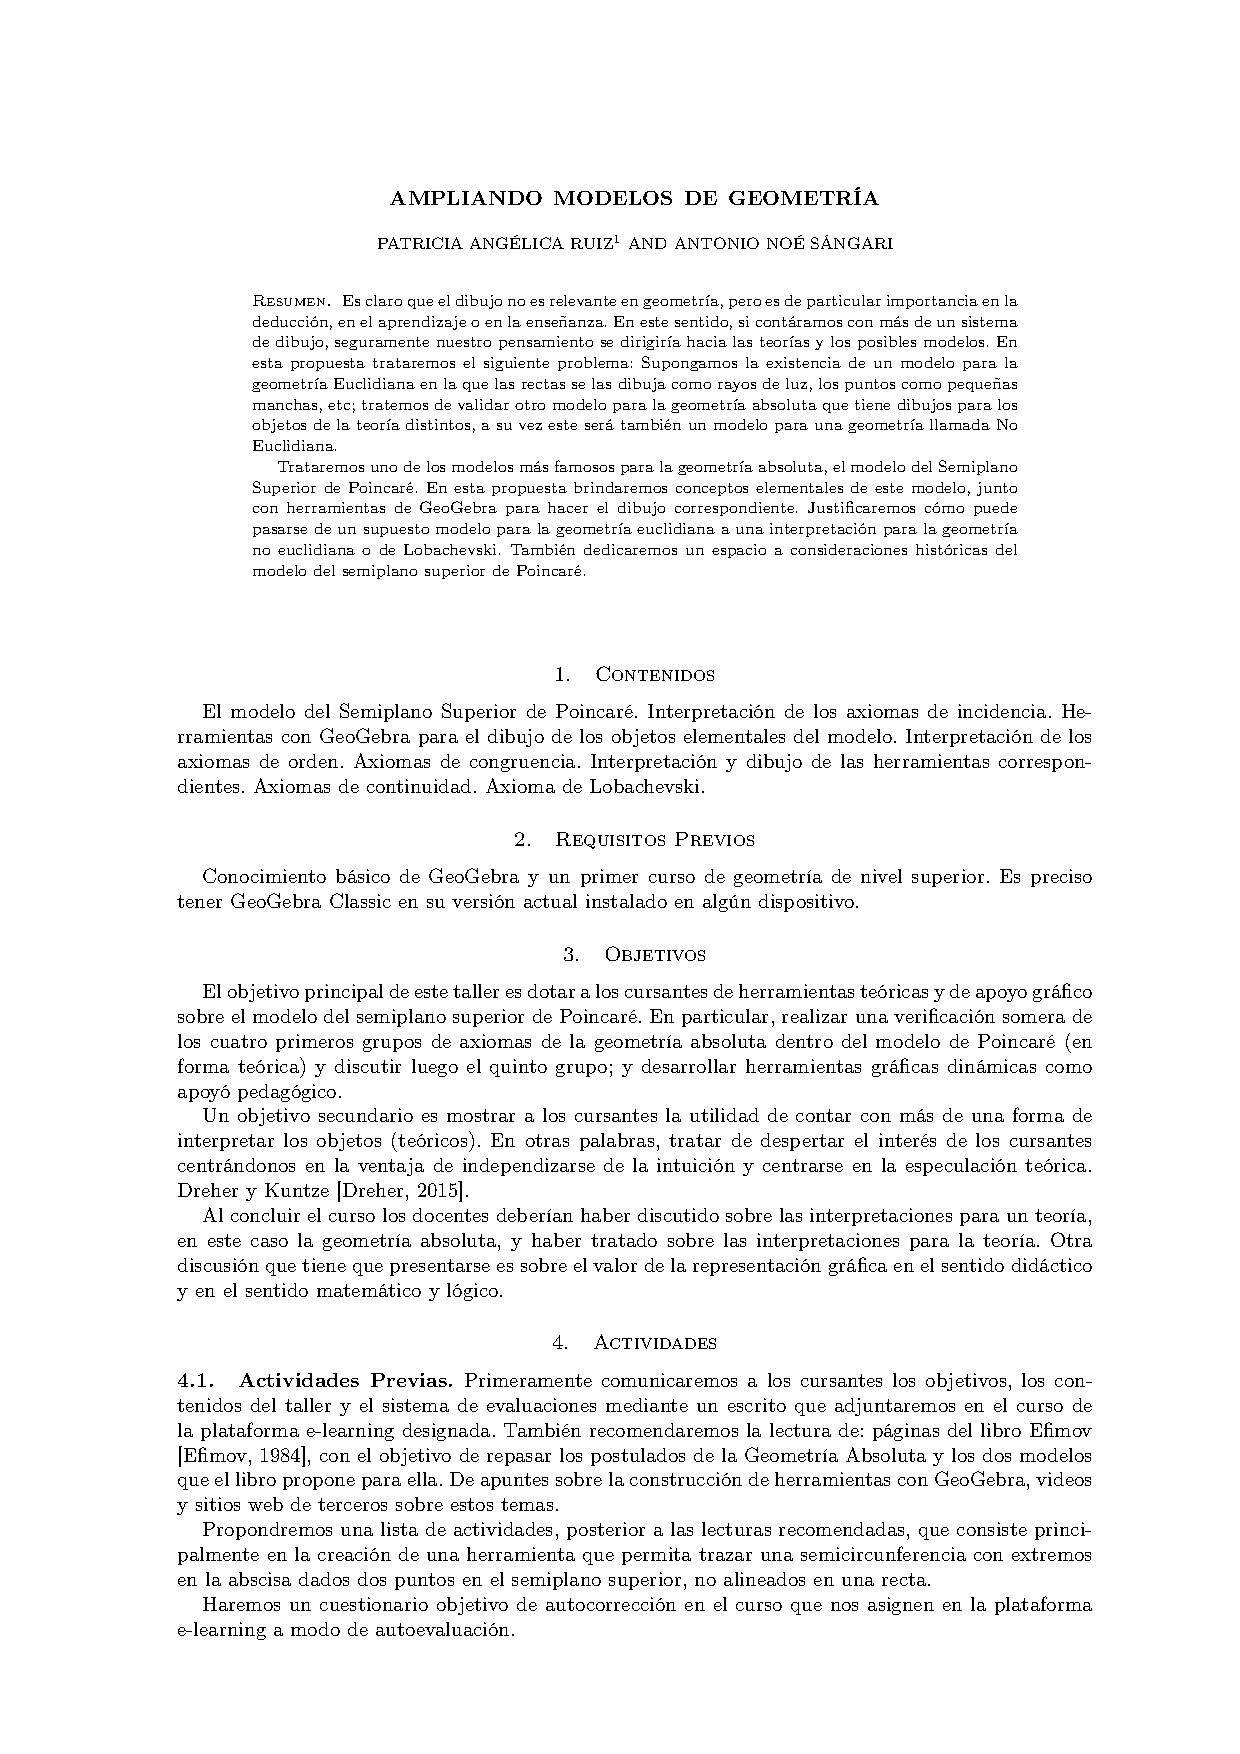
\includepdf[addtotoc={1,section,1,
		{Ampliando Modelos de Geometría}, p1},pages={-},pagecommand={\thispagestyle{fancy}}]{Tall-01/Tall01.pdf}
	\desctotoc{Ruiz, P. A., Sángari, A. N.}
	
	\clearpage
	
	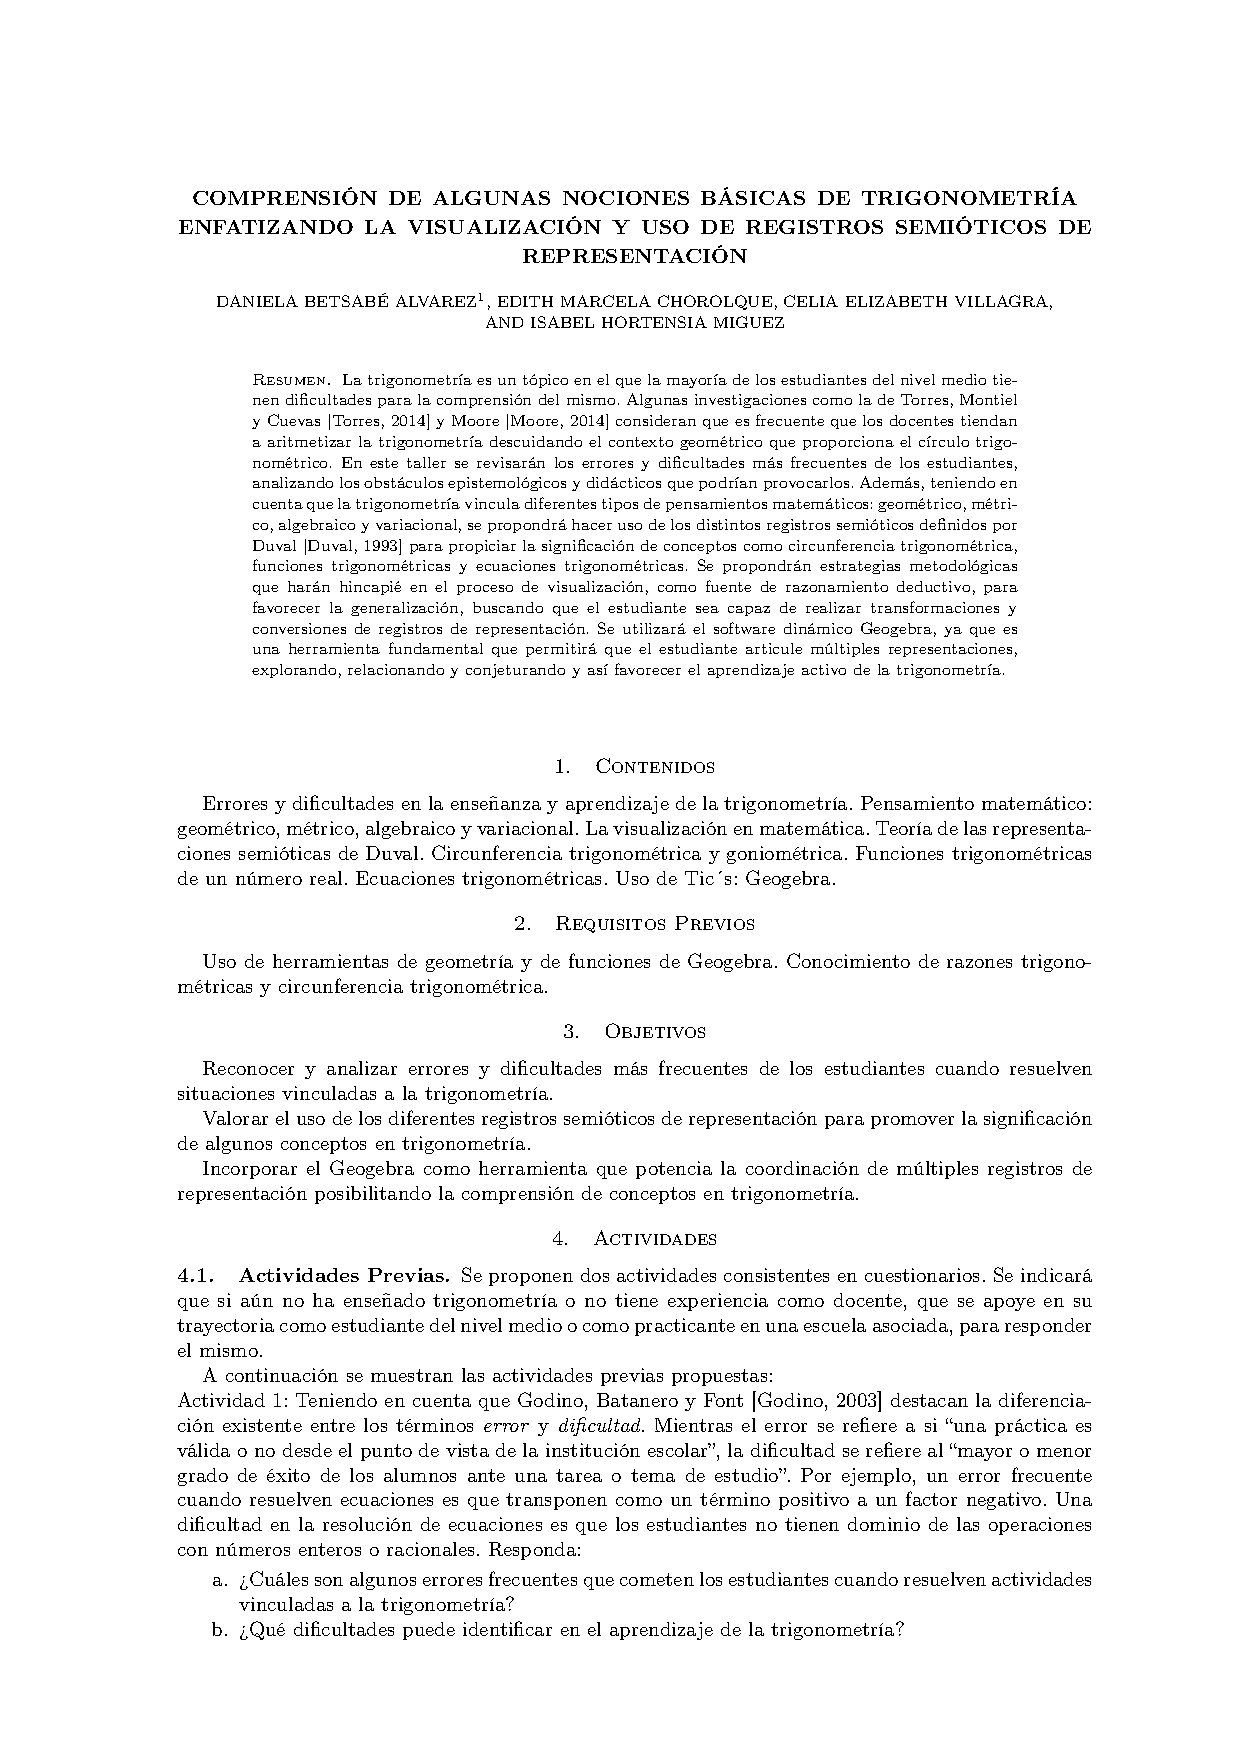
\includepdf[addtotoc={1,section,1,
		{Comprensión de algunas nociones básicas de  trigonometría enfatizando la  visualización y uso de registros semióticos de representación}, p2},pages={-},pagecommand={\thispagestyle{fancy}}]{Tall-02/Tall02.pdf}
	\desctotoc{Alvarez, D.B., Chorolque, E. M., Villagra, C. E., Miguez, I. H.}
		
	\clearpage
	
	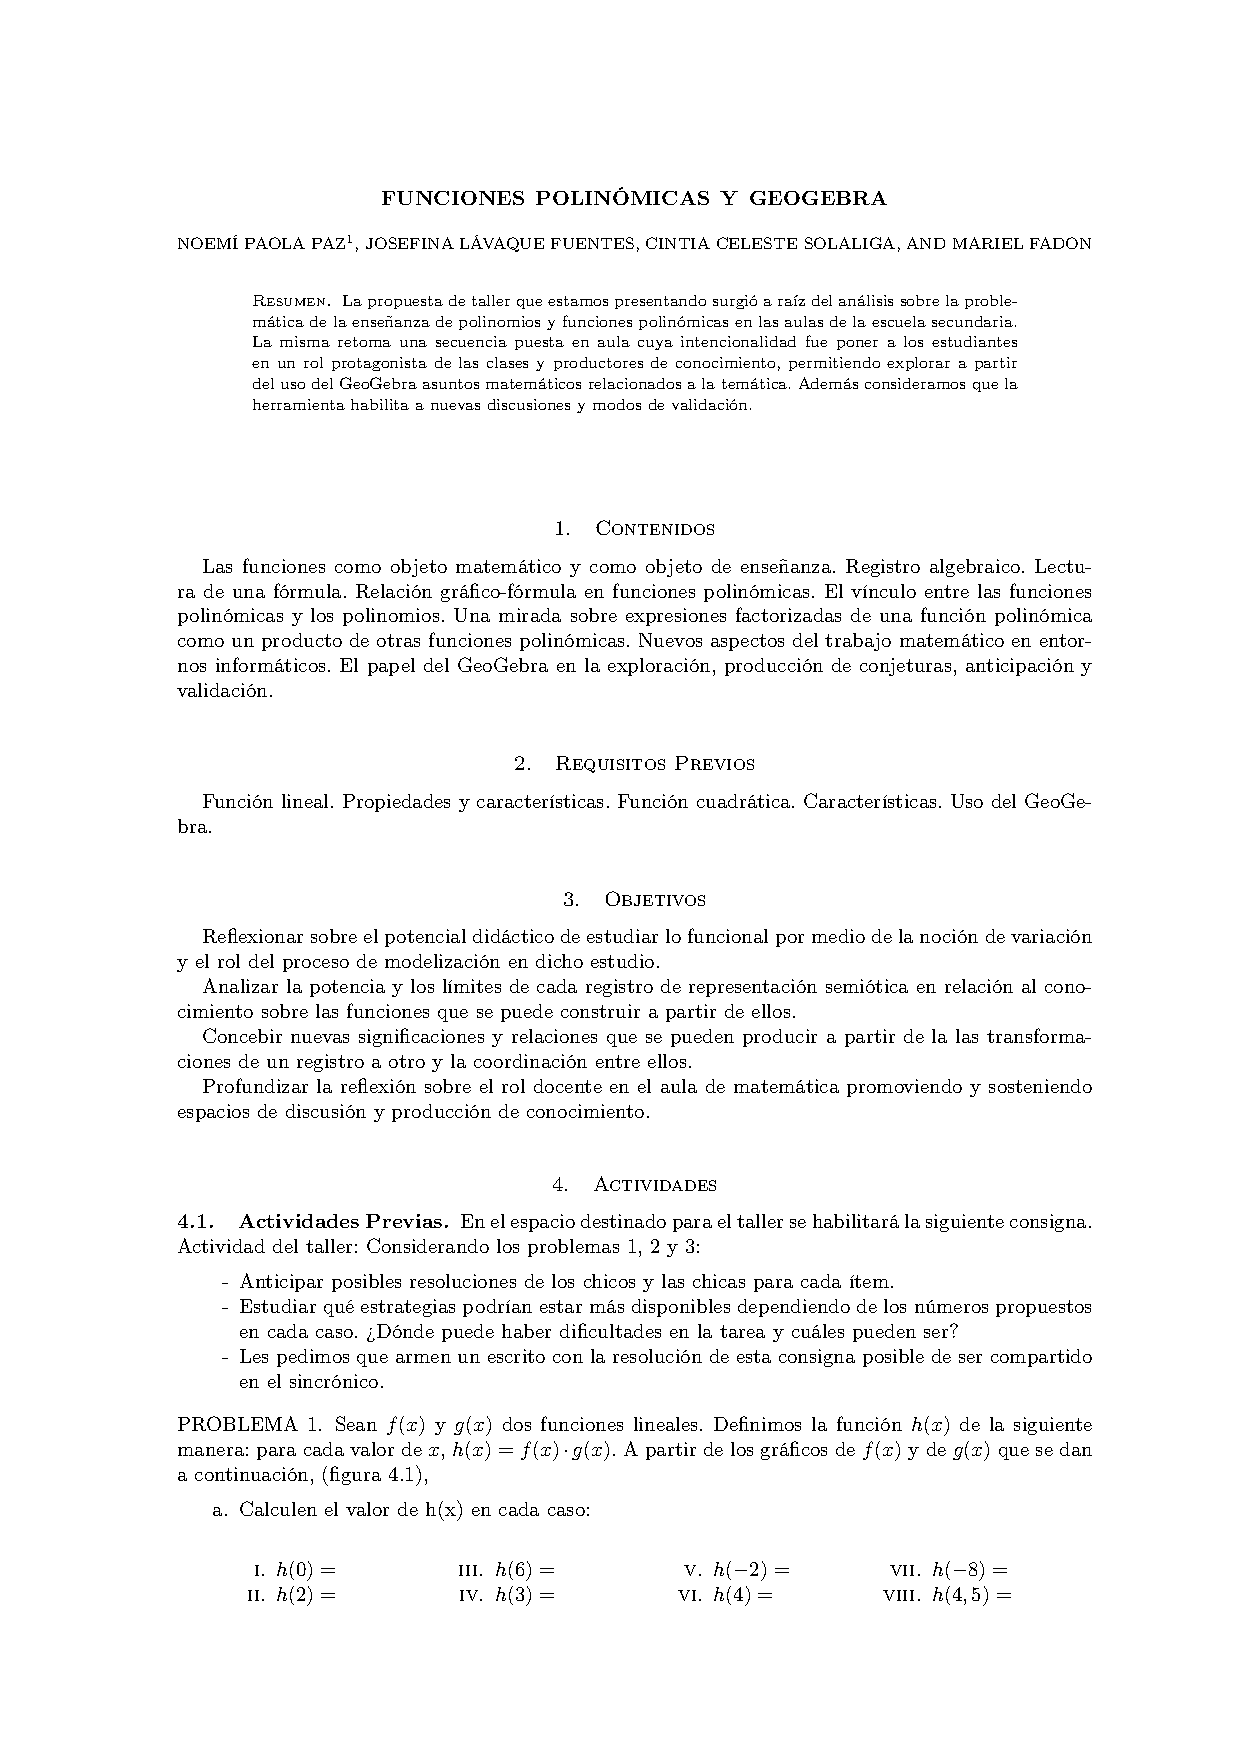
\includepdf[addtotoc={1,section,1,
		{Funciones polinómicas y GeoGebra}, p3},pages={-},pagecommand={\thispagestyle{fancy}}]{Tall-03/Tall03.pdf}
	\desctotoc{Paz, N. P., Fuentes, J. L., Solaliga, C. C., Fadon, M.}
	
	\clearpage
	%------------------------------------------------------------------------------------------------------------
	
	%------------------------------------------------------------------------------------------------------------
	% Comunicaciones breves
	\clearpage
	\vspace*{\fill}
	\begin{center}
		\sffamily \scshape \bfseries \LARGE II
		
		\Huge Comunicaciones breves
	\end{center}
	\vspace*{\fill}
	\addcontentsline{toc}{part}{II \hspace*{1em} Comunicaciones breves}
	\clearpage
	
	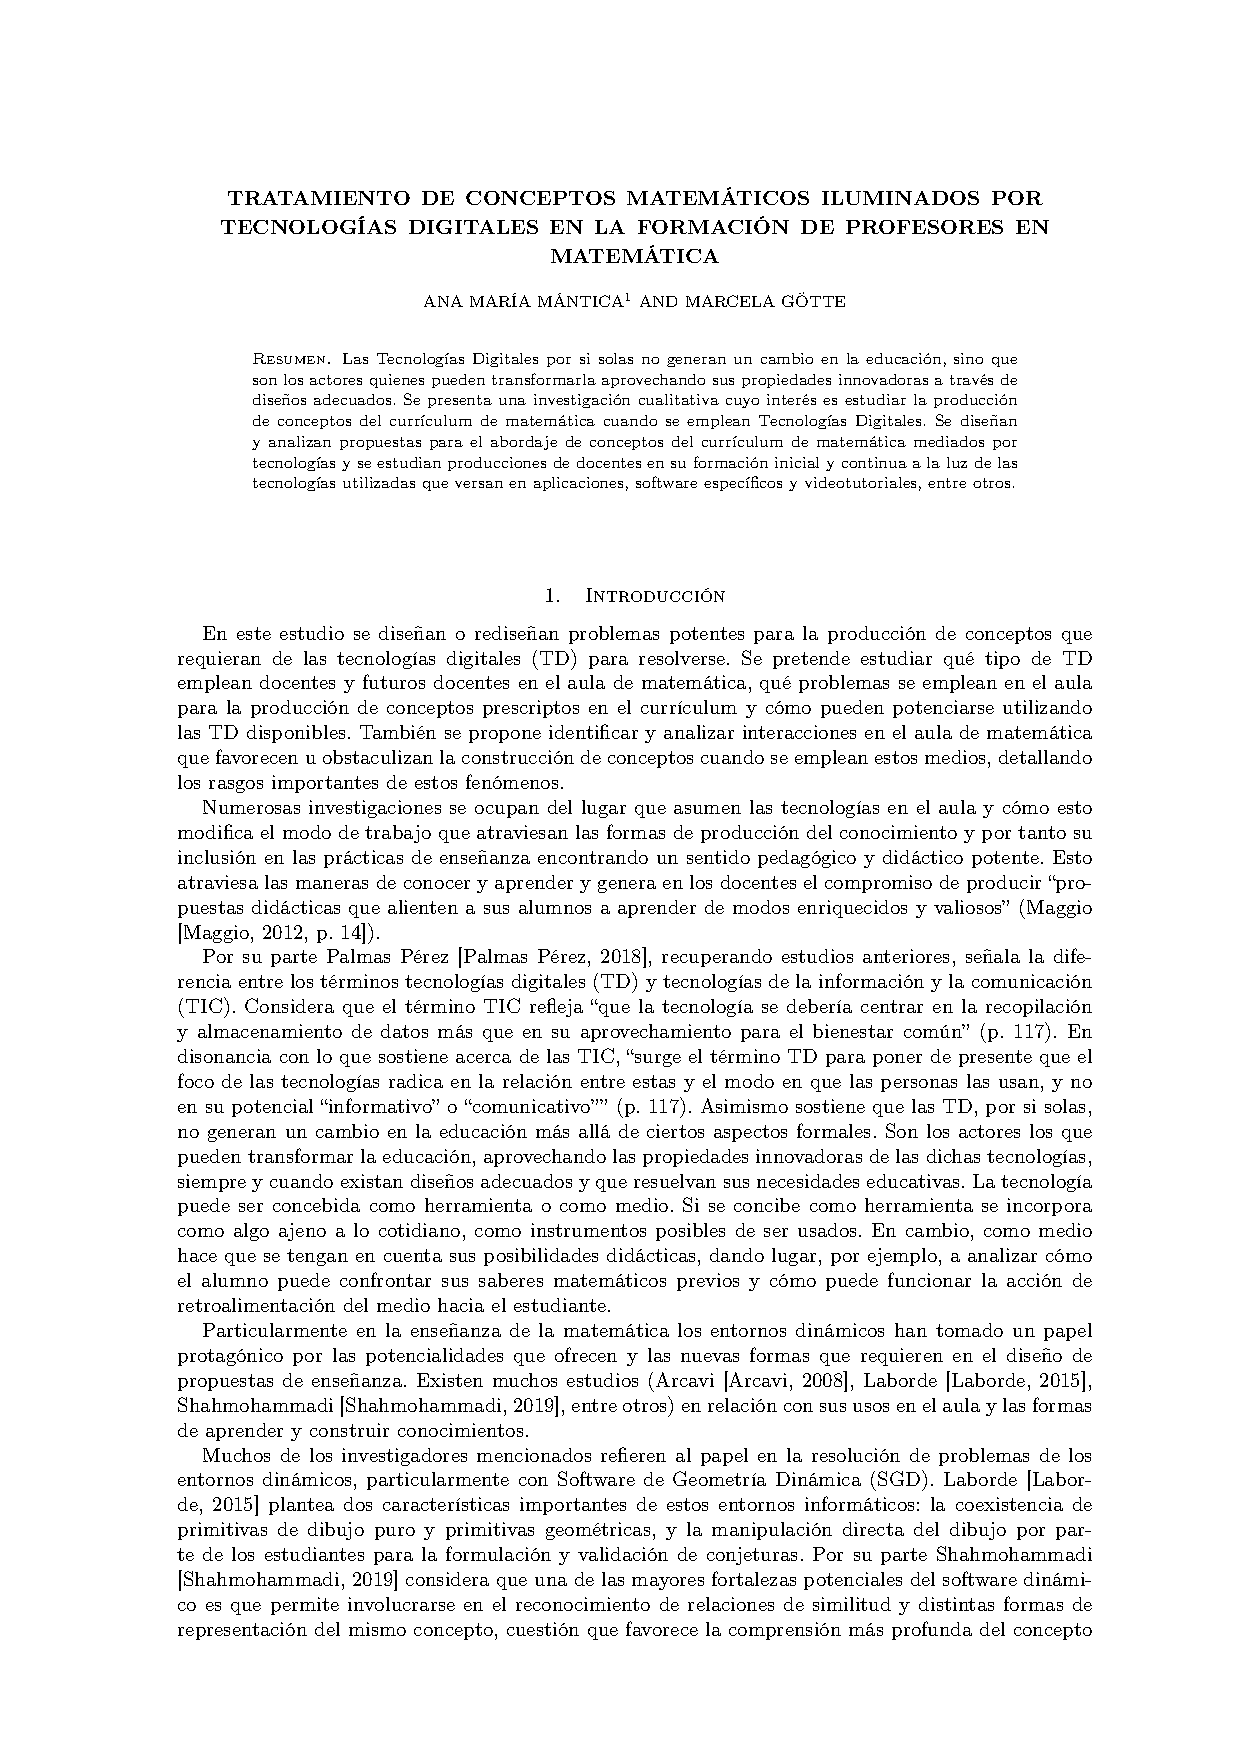
\includepdf[addtotoc={1,section,1,
		{Tratamiento de conceptos matemáticos iluminados por tecnologías digitales en la formación de profesores en matemática}, p4},pages={-},pagecommand={\thispagestyle{fancy}}]{Com-01/Com01.pdf}
	\desctotoc{Mántica, A. M., Götte, M.}
	
	\clearpage
	
	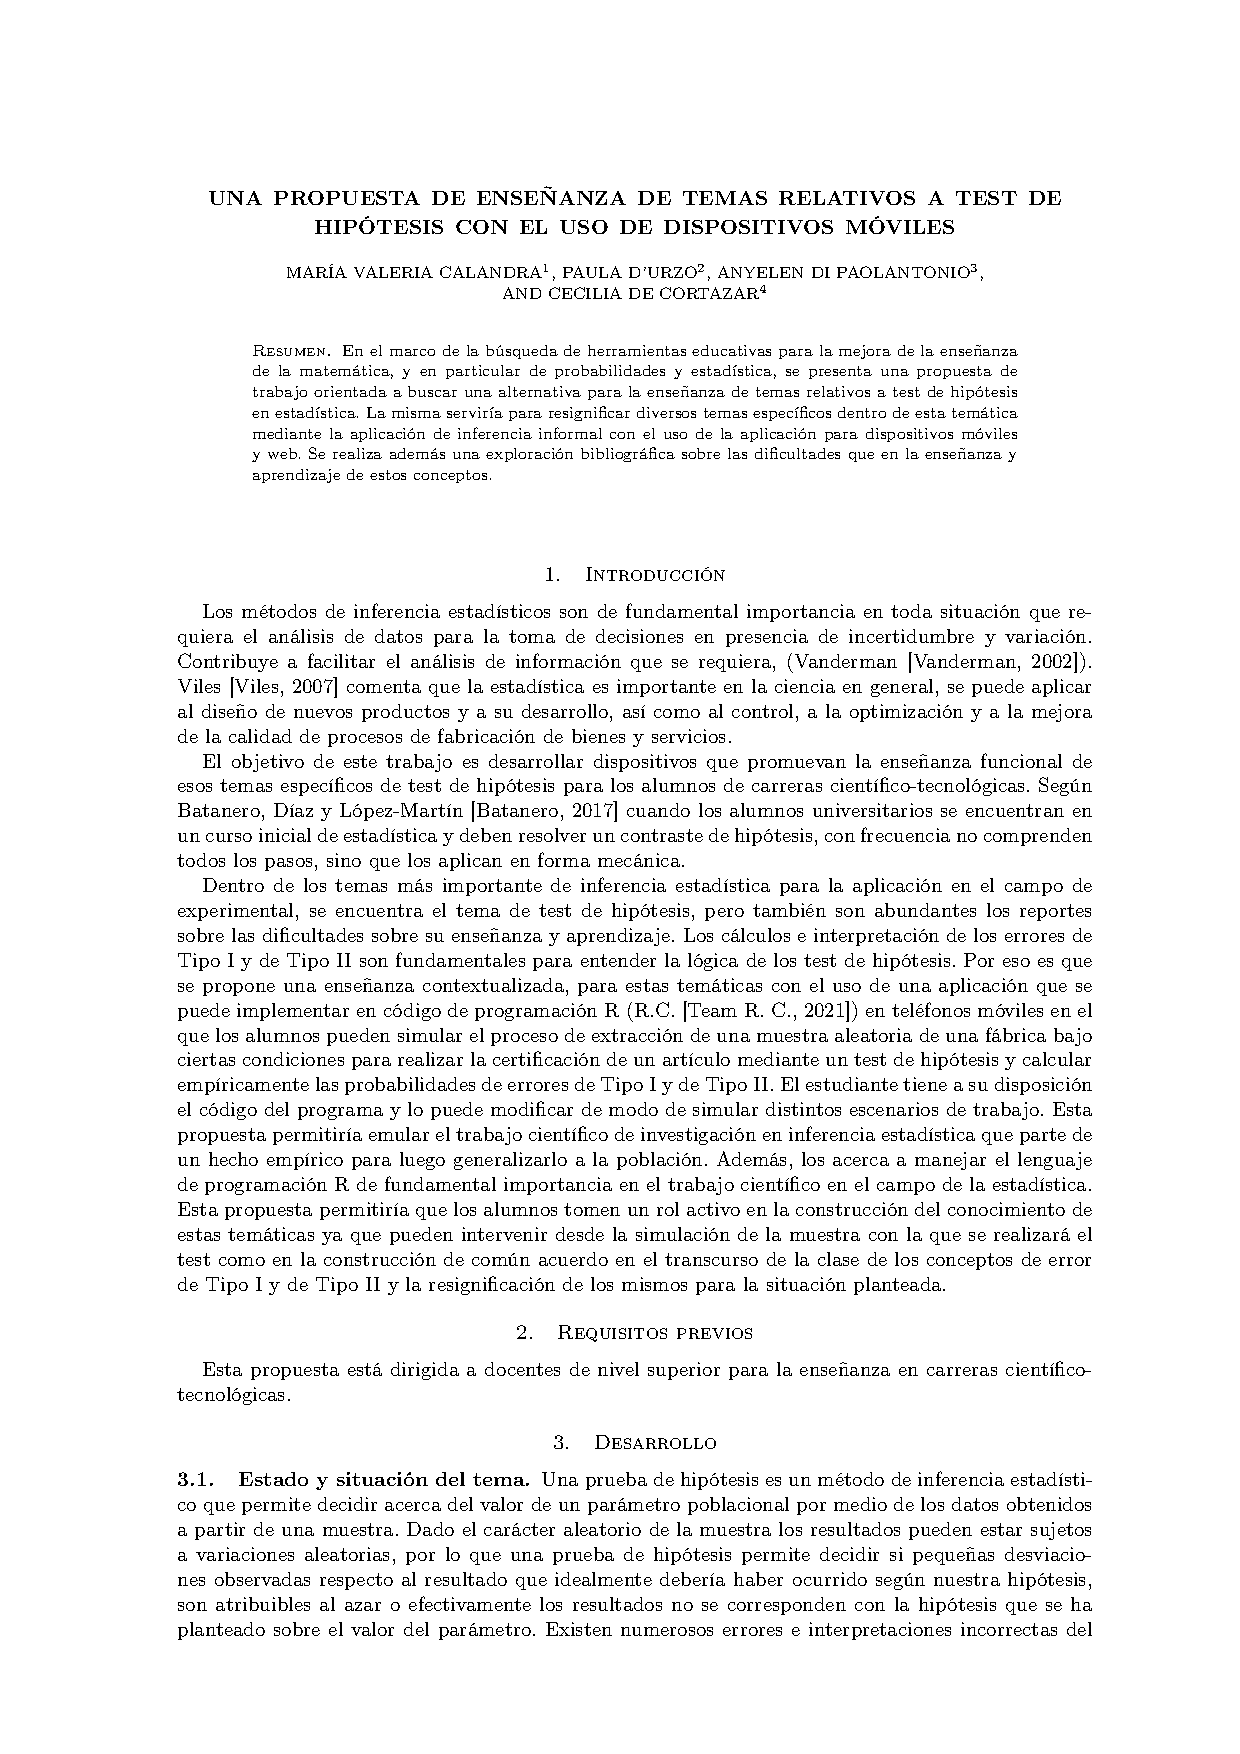
\includepdf[addtotoc={1,section,1,
		{Una propuesta de enseñanza de temas relativos a test de hipótesis con el uso de dispositivos móviles}, p5},pages={-},pagecommand={\thispagestyle{fancy}}]{Com-02/Com02.pdf}
	\desctotoc{Calandra, M. V., D'Urzo, P., Di Paolantonio, A., De Cortazar, C.}
	
	\clearpage
	
	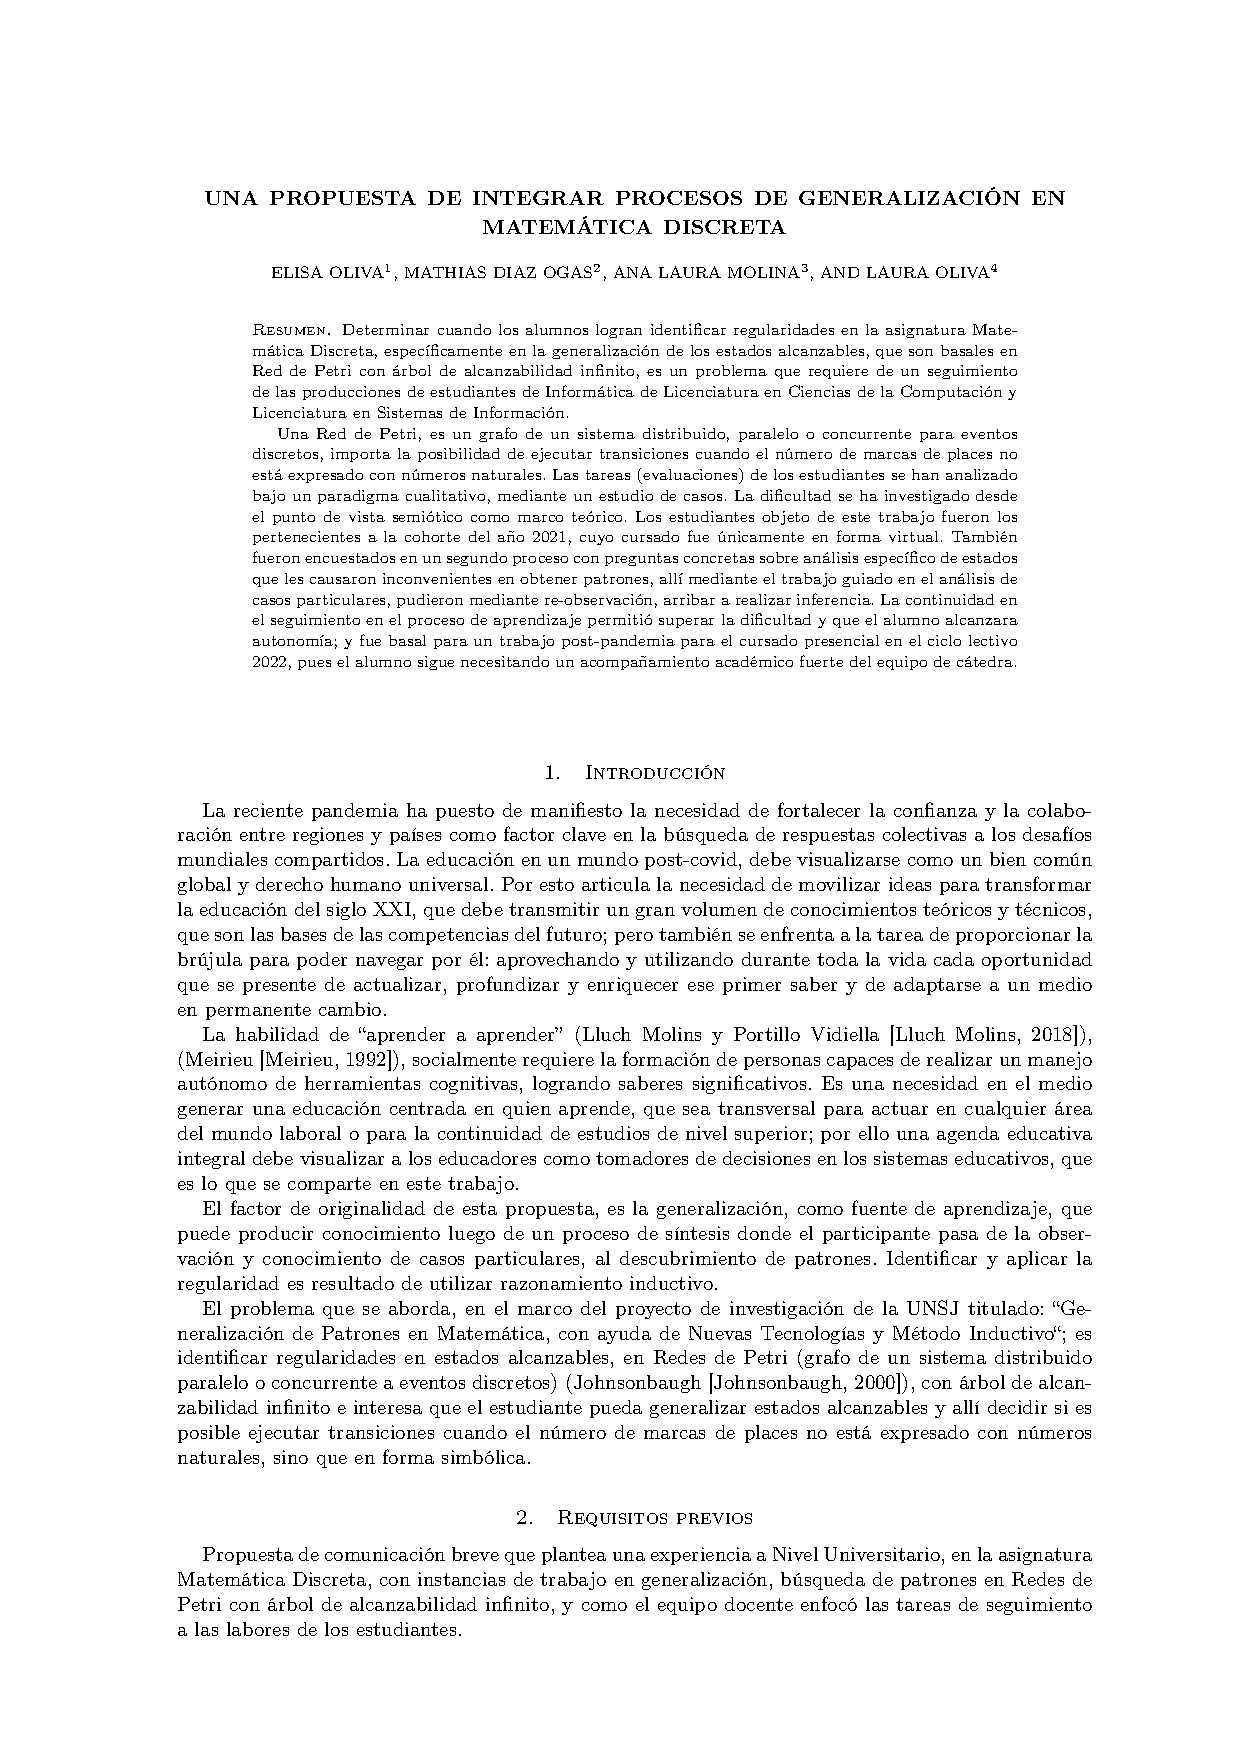
\includepdf[addtotoc={1,section,1,
		{Una propuesta de integrar procesos de generalización en Matemática Discreta}, p6},pages={-},pagecommand={\thispagestyle{fancy}}]{Com-03/Com03.pdf}
	\desctotoc{Oliva, E., Diaz Ogas, M., Molina, A. L., Oliva, L.}
	
	\clearpage
	
	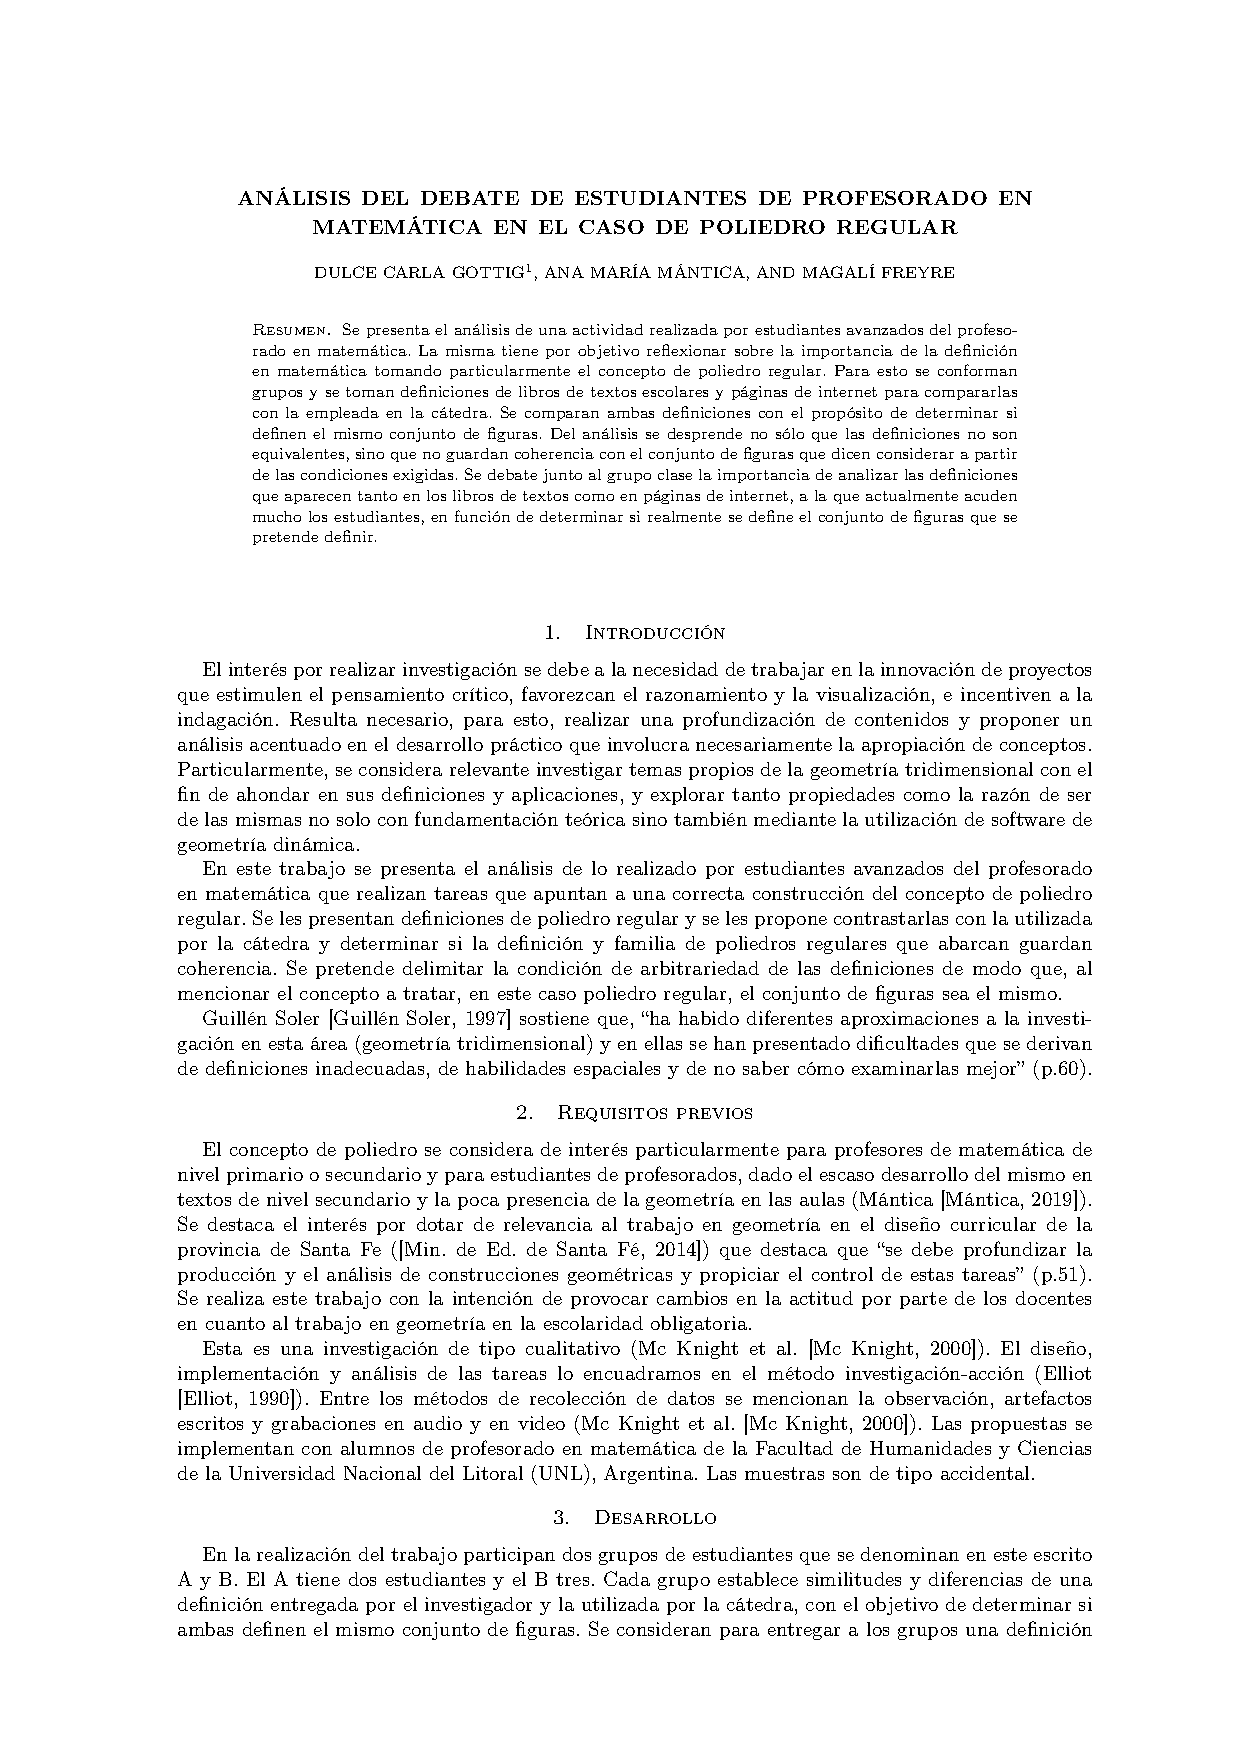
\includepdf[addtotoc={1,section,1,
		{Análisis del debate de estudiantes de profesorado en matemática en el caso de poliedro regular}, p7},pages={-},pagecommand={\thispagestyle{fancy}}]{Com-04/Com04.pdf}
	\desctotoc{Gottig, D. C., Mántica, A. M., Freyre, N.}
	
	\clearpage
	
	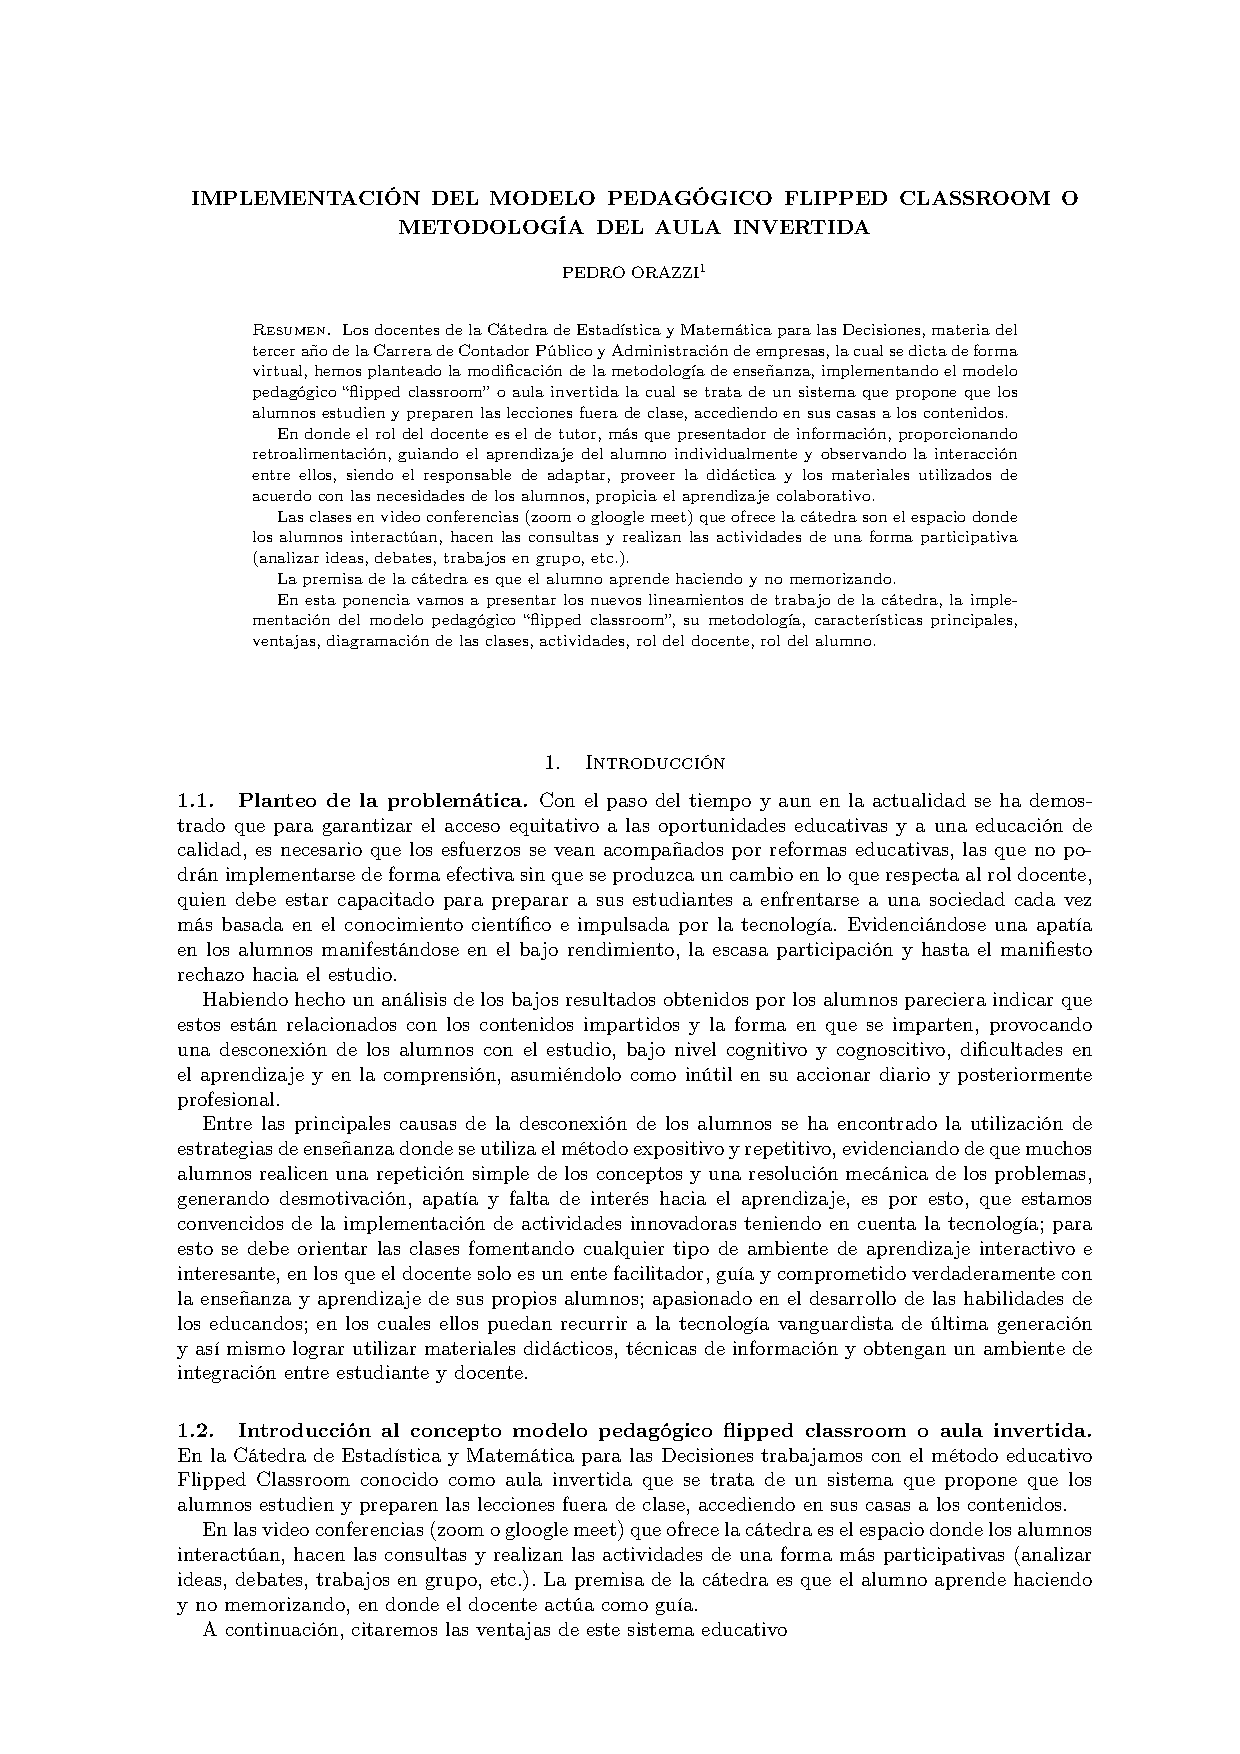
\includepdf[addtotoc={1,section,1,
		{Implementación del modelo pedagógico flipped classroom o metodología del aula invertida}, p8},pages={-},pagecommand={\thispagestyle{fancy}}]{Com-05/Com05.pdf}
	\desctotoc{Orazzi, P.}
	
	\clearpage
	
	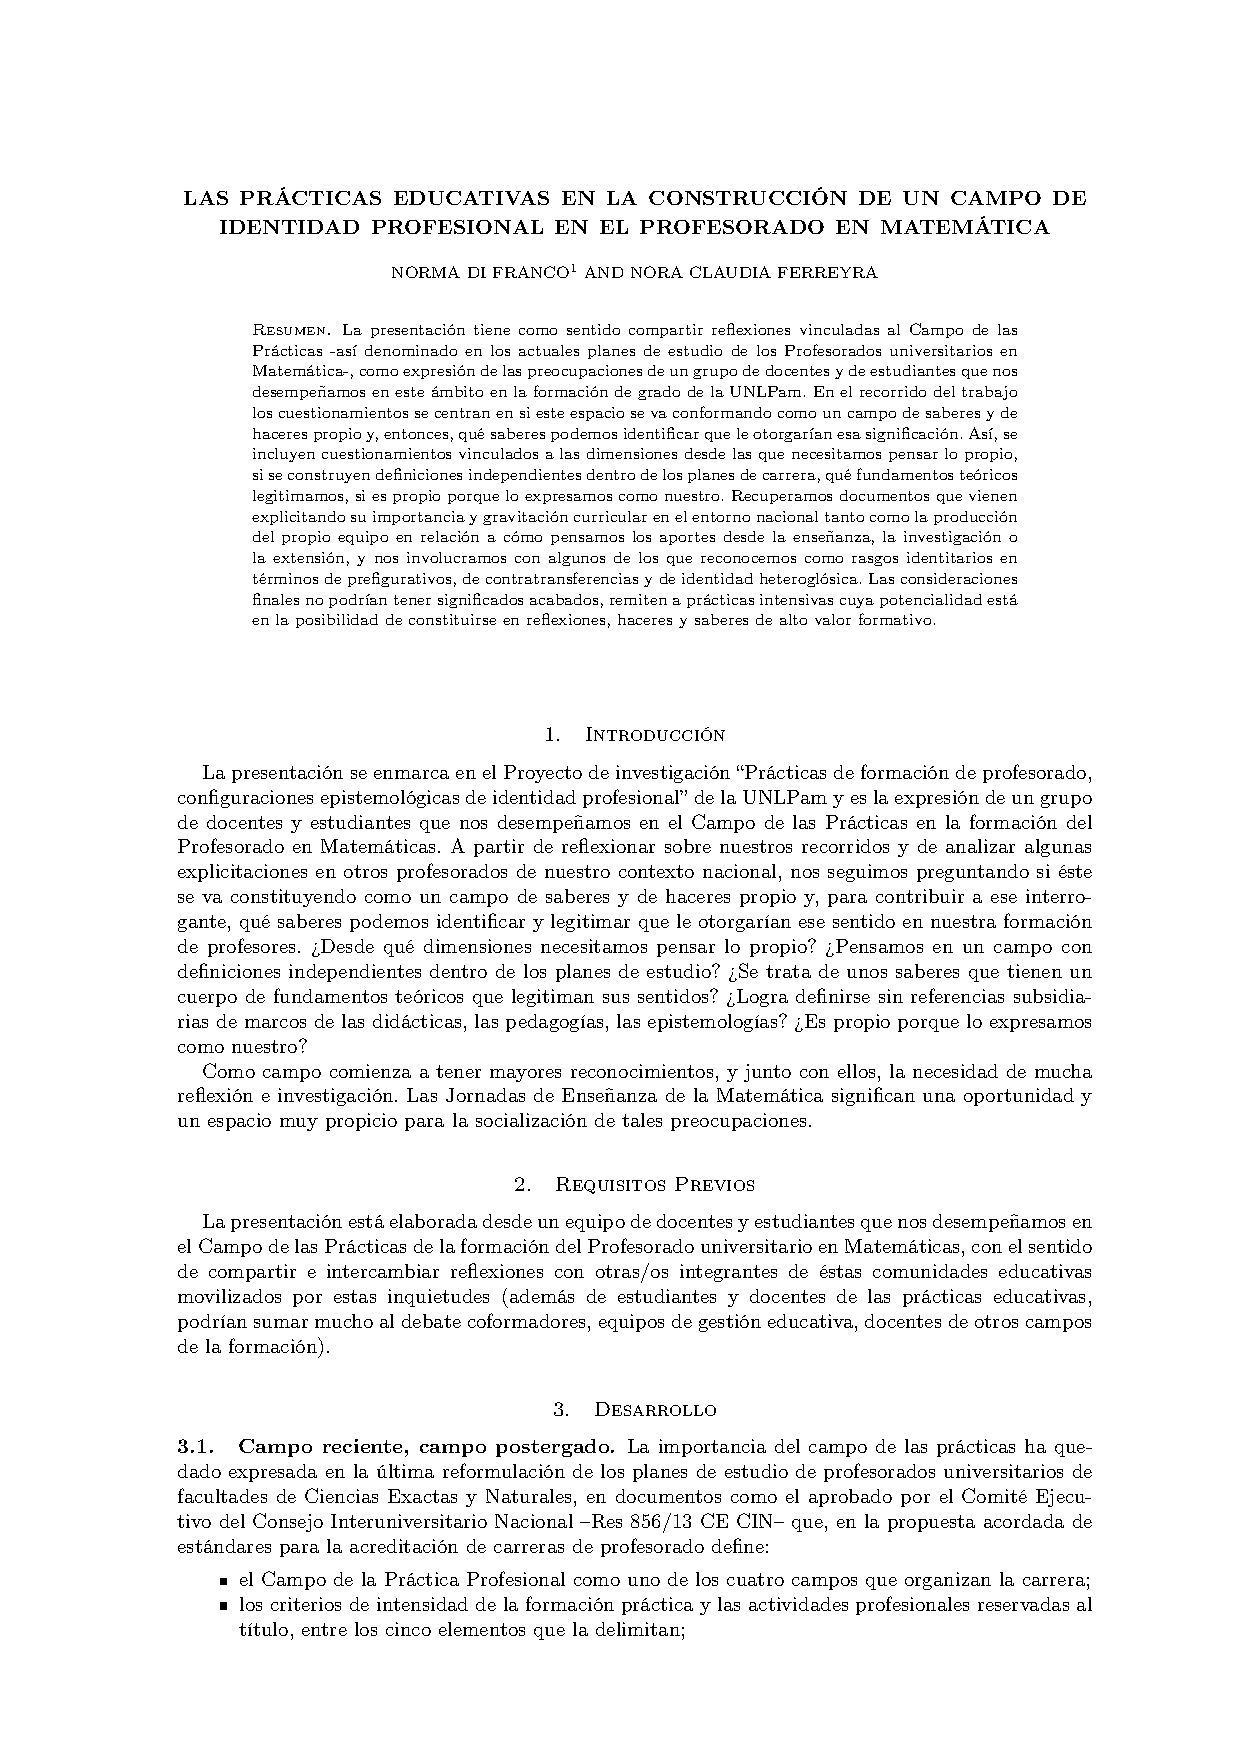
\includepdf[addtotoc={1,section,1,
		{Las Prácticas educativas en la construcción de un campo de identidad profesional en el Profesorado en Matemática}, p9},pages={-},pagecommand={\thispagestyle{fancy}}]{Com-06/Com06.pdf}
	\desctotoc{Di Franco, N., Ferreyra, N. C.}
		
	\clearpage
	
	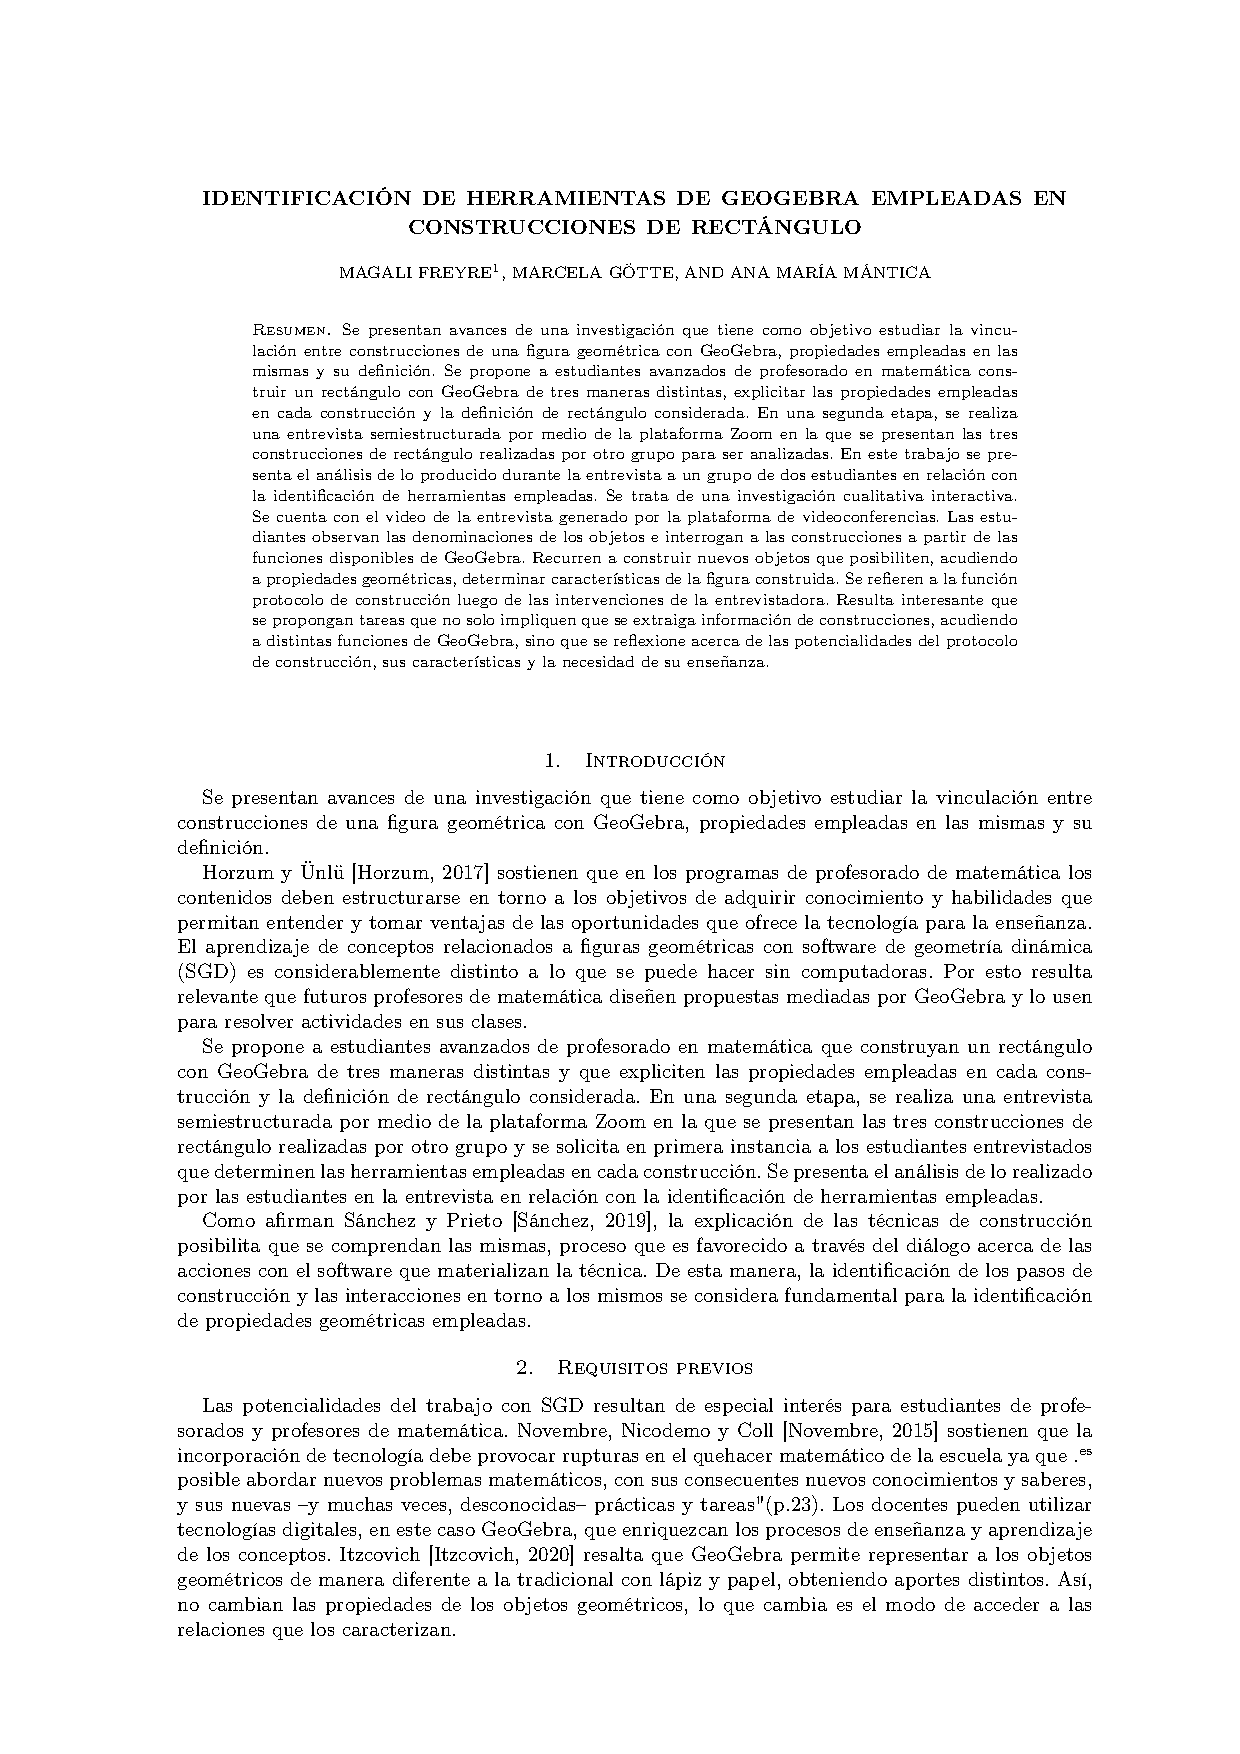
\includepdf[addtotoc={1,section,1,
		{Identificación de herramientas de GeoGebra empleadas en construcciones de rectángulo}, p10},pages={-},pagecommand={\thispagestyle{fancy}}]{Com-07/Com07.pdf}
	\desctotoc{Freyre, M., Götte, M., Mántica, A. M.}
	
	\clearpage
	
	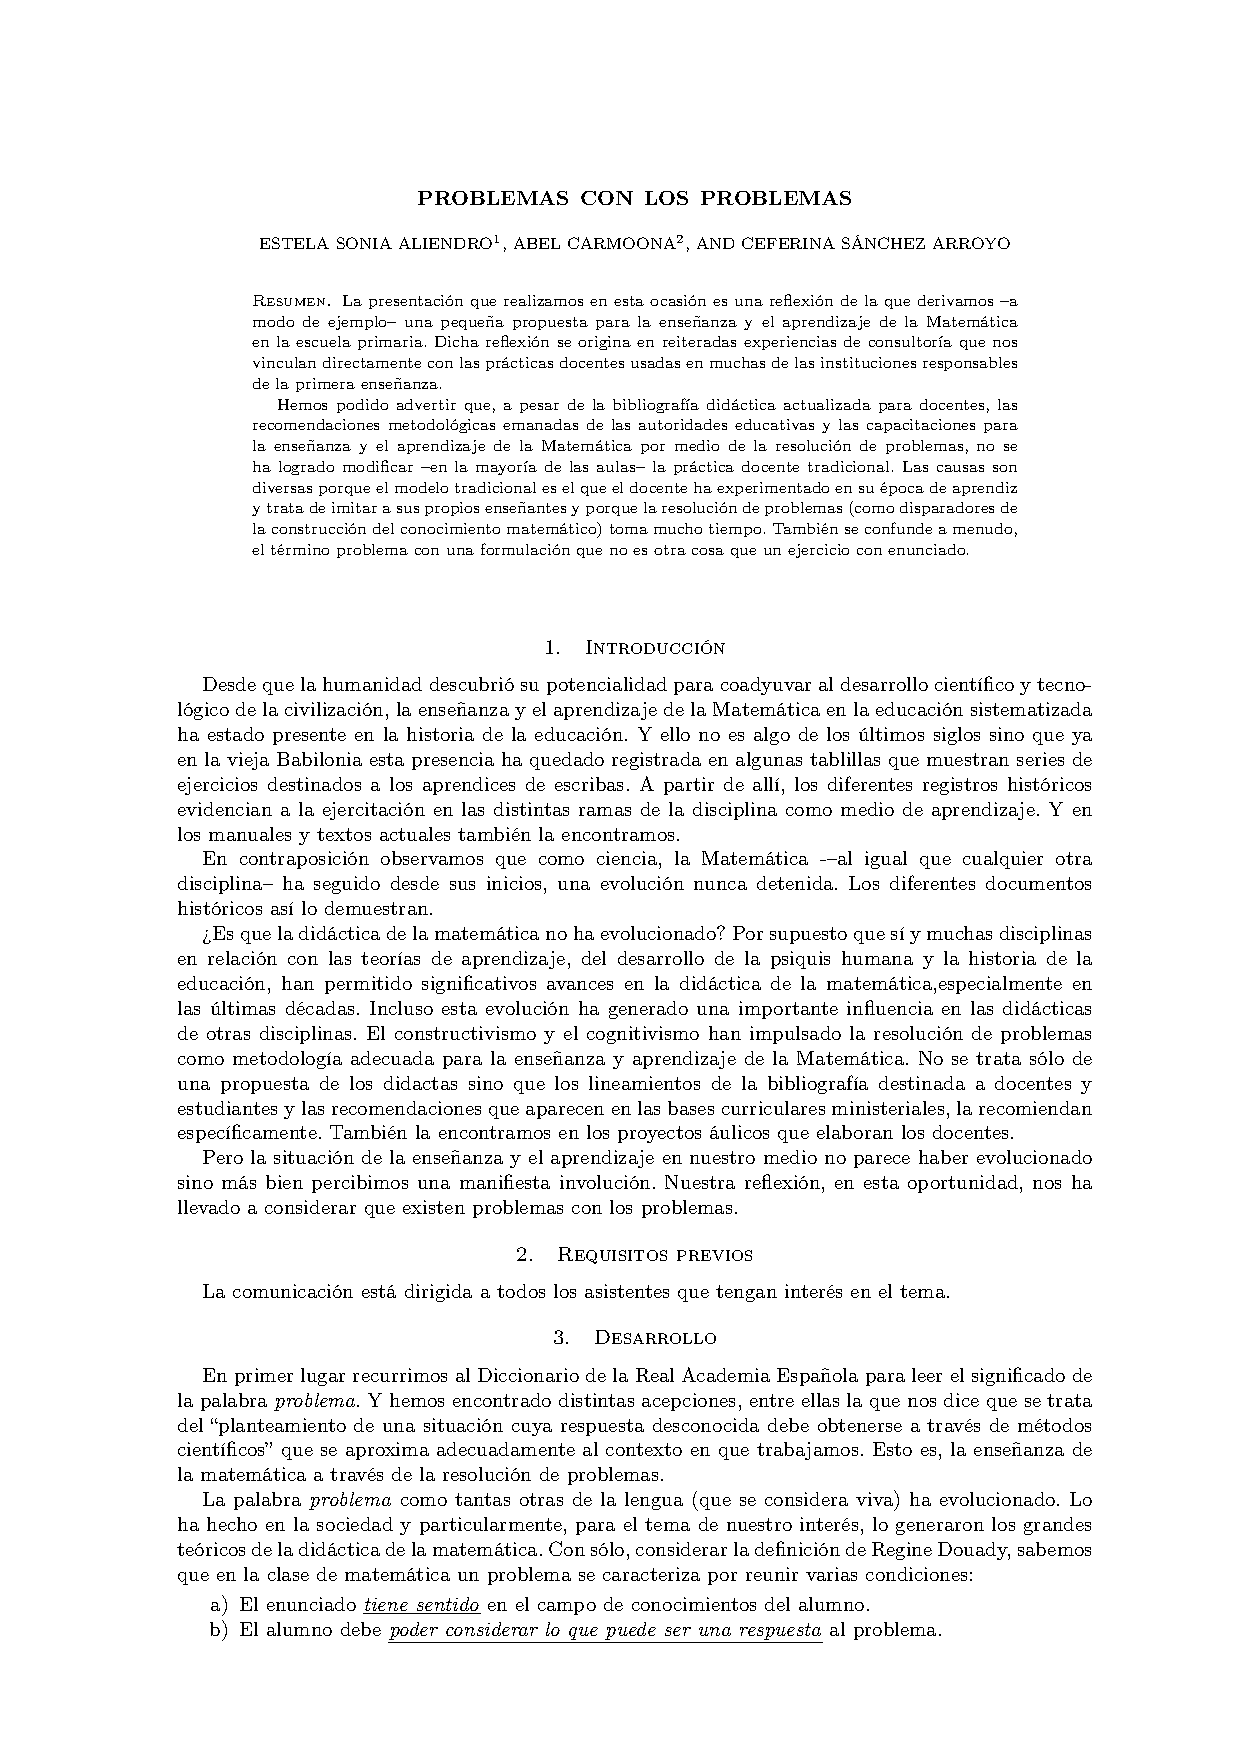
\includepdf[addtotoc={1,section,1,
		{Problemas con los Problemas}, p11},pages={-},pagecommand={\thispagestyle{fancy}}]{Com-08/Com08.pdf}
	\desctotoc{Aliendro, E. S., Carmoona, A., Sánchez Arroyo, C.}
	
	\clearpage
	%------------------------------------------------------------------------------------------------------------
	
	
\includepdf{Contraportada.pdf}
\end{document}